\documentclass{guide}
\usepackage{caption, graphicx}

\title{Solderen}
\level{2}

\begin{document}
Op het moment dat je een project op een breadboard permanent wil maken, zul je moeten gaan solderen. Ook het verwijderen en toevoegen van pinnen, het toevoegen van bedrading, of het maken van een breakout (een adapter voor een chip zodat je deze kan gebruiken op een breadboard) zul je moeten doen door te solderen.
\section{Tools}
Voor het solderen heb je verschillende dingen nodig:

\paragraph{Soldeerbout} Op het lab zijn verschillende soldeerbouten aanwezig. Let goed op dat je de juiste soldeerbout kiest voor de juiste tin. Op het moment dat je deze aanzet duurt het een tijdje voordat ze opgewarmd zijn. Dit kan je testen door een beetje tin tegen de punt aan te houden. Smelt de tin dan is de soldeerbout klaar voor gebruik.

\paragraph{Tin} Op het lab zijn 2 verschillende soorten tin aanwezig. Lood vrij en met lood. Lood tin heeft een lagere smelt temperatuur en vloeit makkelijker. Lood vrij tin is beter voor je gezondheid en het vloeien kan verbeterd worden met flux.

\paragraph{Flux} Flux is een stof die er voor zorgt dat de oxidatielaag (roest) op het metaal verwijdert wordt, waardoor de soldeer tin beter kan vloeien en hechten. Smeer een klein beetje flux met het kwastje op de aanhechtingspunten. Veeg na het gebruik de resten flux van de pcb af.

\paragraph{Afzuiging}
Bij het solderen komen schadelijke dampen vrij. Gebruik hierom ALTIJD de afzuiging en plaats deze ~10cm boven het project.
\subsection{Extra tools}

\paragraph{Solder wick \& Soldeer zuiger}
Deze tools kunnen gebruikt worden om tin weer weg te halen. Solder wick gebruik je door het op de tin te leggen en dan warm te maken met de soldeerbout. Zodra de tin gesmolten is haal je de wick er af. De tin blijft hier aan plakken. Om de zuiger te gebruiken, maak je de tin eerst vloeibaar (met de soldeerbout), vervolgens houd je de zuiger bij de tin en druk je op de knop. De tin wordt dan opgezogen.

\paragraph{Sponsjes}
Bij de soldeerbout liggen verschillende sponsjes (metalen en natuurlijke varianten). Gebruik deze om overtollig soldeer tin van je soldeerbout af te halen. Als je een natuurlijke spons gebruikt moet je er voor zorgen dat deze nat is.

\paragraph{3e handje \& Loep}
Een 3e hand kan gebruikt worden om je project vast te houden, dit houdt je werk en componenten stabiel. De loep kan je gebruiken om kleine details te zien tijdens het solderen of om je connectie te controleren

\newpage
\section{Solderen}
Nu we alle tools kennen kunnen we beginnen met solderen.\\

\subsection{Tips}
\begin{minipage}{.50\textwidth}
  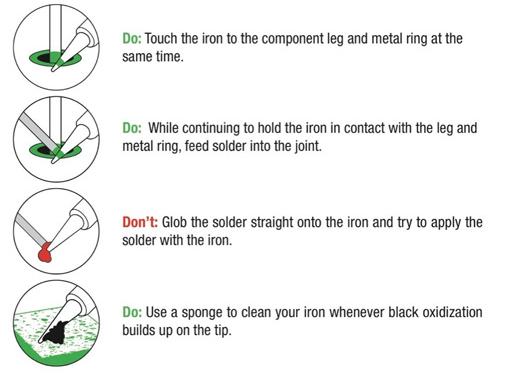
\includegraphics[width=\textwidth]{images/dosanddonts.png}
  \captionof{figure}{Do's and Dont's van solderen}\label{fig:1}
\end{minipage}
\begin{minipage}{.50\textwidth}
  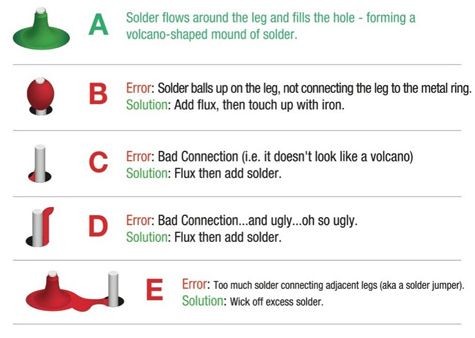
\includegraphics[width=\textwidth]{images/correct_joint.png}
  \captionof{figure}{Correcte en Incorrecte soldeer joints}\label{fig:2}
\end{minipage}

\subsection{Instructies}
\begin{minipage}{.60\textwidth}
  \begin{enumerate}
  \item Lees deze instructies volledig door.
  \item Plaats het component op de juiste manier op / in het pcb.
  \item Als je flux wilt gebruiken smeer dat nu op de pad.
  \item Maak de tip van de soldeerbout schoon.
  \item Warm de pad op de pcb en de pin van het component op met de sweetspot van de soldeerbout (zie hiernaast) voor 1 seconden.
  \item Voeg, terwijl je de soldeerbout er op blijft houden langzaam een klein beetje tin toe. De tin moet op de pad vast smelten.
  \item Haal de tin-draad weg en hou de bout nog 1 seconde op de joint.
  \item Haal de soldeerbout weg en check de joint met figuur \ref{fig:1}.
  \item Is alles gesoldeerd, zet dan de soldeerbout uit. Als je met lood hebt gesoldeerd was dan ook je handen.
  \end{enumerate}
\end{minipage}
\begin{minipage}{.40\textwidth}
  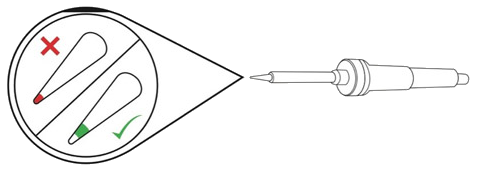
\includegraphics[width=\textwidth]{images/iron_hotspot.png}
  \captionof{figure}{Soldeerbout hotspot.}\label{wrap-fig:1}
\end{minipage}




\end{document}
